\section{Task: Associate ARTAS TRIs}
\label{sec:task_associate_artas_tris}

This task allows creation of UTNs and target report association based on ARTAS tracks and the TRI information.

Please note that if no ARTAS TRI SPF information exists in the database, these steps do not have to be performed.\\

\begin{figure}[H]
  \hspace*{-2.5cm}
    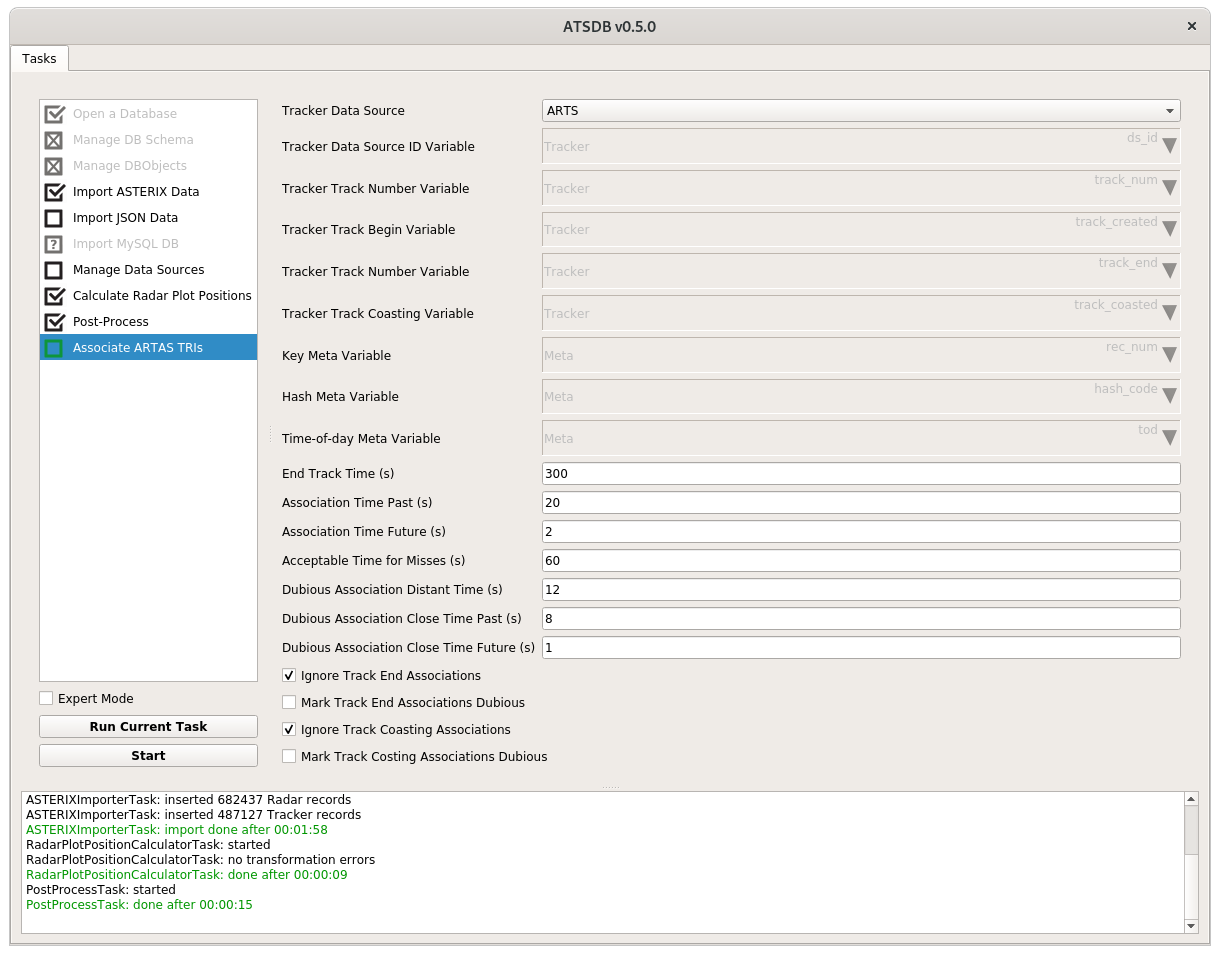
\includegraphics[width=19cm]{figures/artas_association_config.png}
  \caption{Task: Associate ARTAS TRIs}
\end{figure}

In this task, the ARTAS association information stored in system track updates can be used to create UTN which associate each system track update to the used sensor target reports.

The following configuration options exist

\begin{itemize}  
\item Tracker Data Source: Name of tracker data source from which associations shall be created.
\item Data Variables: Definition of variables to be used in processing. Does not have to be changed.
\item End Track Time (s): Track update gap time (in seconds) after which a new UTN will be created (even if no track begin/end flag is set).
\item Association Time Past (s): Time window length (in seconds) into the past where sensor target reports are considered for association.
\item Association Time Future (s): Time window length (in seconds) into the future where sensor target reports are considered for association.
\item Acceptable Time for Misses (s): Time window length at the beginning and end of the recording (in seconds) where misses (not found hash codes) are acceptable.
\item Dubious Association Distant Time (s): Maximum age of made associations (in seconds), if older they are considered as dubious associations.
\item Dubious Association Close Time Past (s): Time window length (in seconds) into the past where made associations are considered as dubious if multiple sensor hashes exist.
\item Dubious Association Close Time Future (s): Time window length (in seconds) into the future where made associations are considered as dubious if multiple sensor hashes exist.
\item Ignore Track End Associations: If set, no assocations for system track updates where the track end flag is set are created.
\item Mark Track End Associations Dubious: If set, assocations for system track updates where the track end flag is set are counted as dubious.
\item Ignore Track Coasting Associations: If set, no assocations for system track updates where the track coasted flag is set are created.
\item Mark Track Coasting Associations Dubious: If set, assocations for system track updates where the track coasted flag is set are counted as dubious.
\end{itemize}

\paragraph{UTN Creation from System Track Numbers and End Track Time}: 

The task should create a unique target number (UTN) for every ARTAS track. The track begin/end flags therefore are used to create new UTNs or finalize existing ones. To cover the case when such information is wrong or missing, the 'End Track Time' is used to check the time between track updates from one track number. If the gap is larger then the defined time, a new UTN is created even if no track begin/end flag was set.

\paragraph{Association Time Window}

Consider the following figure: In a timeline, a system track update exists at time \textbf{0}, while referenced sensor target reports exist at the times \textbf{1,2,3}. In this description, it is assued that all sensor target reports have the same referenced ARTAS MD5 hash value.


\begin{figure}[H]
  \center
    
\includegraphics[width=8cm]{figures/artas_assoc_timeline.png}
\end{figure}


The time window defined by [\textit{Association Time Past, Association Time Future}] defines which referenced sensor target reports are considered for association. The 'Past' time is the time difference into the past (default 20s), the 'Future' time is the time difference into the future (default 2s). \\

In this example, 1 and 2 are considered, while 3 is disregarded. Since 1 is closer in time to the system track update, the association between (0,1) is made.

\begin{figure}[H]
  \center
    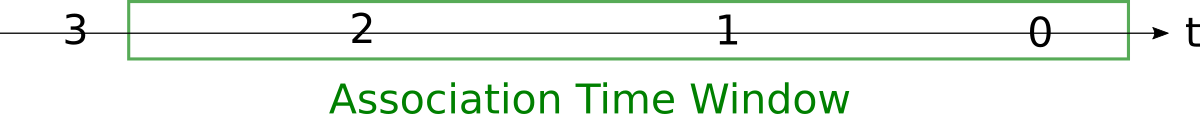
\includegraphics[width=8cm]{figures/artas_assoc_window.png}
\end{figure}

The time defined by \textit{Dubious Association Distant Time} is used to mark assocations which are older than the defined time as dubious. The associations are still created, but counted as dubious. Since 2 is still in the association time window, the assocation (0,2) is made but counted as dubious.

\begin{figure}[H]
  \center
    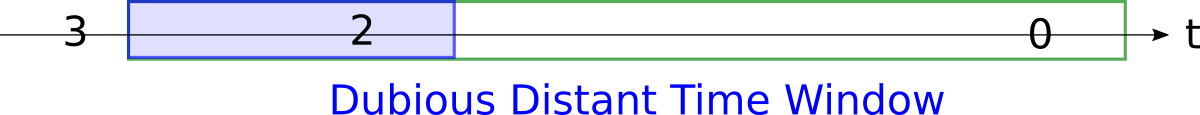
\includegraphics[width=8cm]{figures/artas_assoc_dubious_distant_window.png}
\end{figure}


The time window defined by [\textit{Dubious Association Close Time Past, Dubious Association Close Time Future}] defines when assocations are counted as dubious if multiple referenced sensor target reports exist in it. In this case, 1 and 2 are considered for association, and since 1 is closer in time to the system track update, the association between (0,1) is made. But, since 2 also falls into this time window, the association of (0,1) is counted as dubious association.

\begin{figure}[H]
  \center
    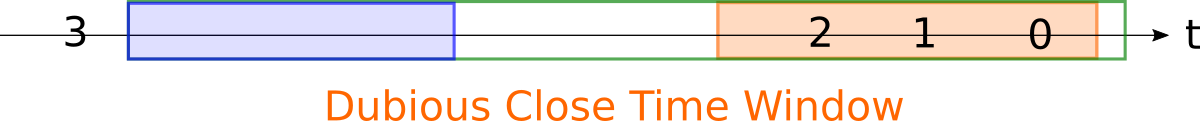
\includegraphics[width=8cm]{figures/artas_assoc_dubious_close_window.png}
\end{figure}


\paragraph{Ignore Track End/Coasting Associations}

Currently in ARTAS, (according to the authors information) track end or coasted updates contain wrong TRI information (from previous updates). If the respective checkboxes are set, this TRI information is disregarded. If they are not checked, the associations are made and can be investigated.

\paragraph{Running}

Using the 'Run Current Task' button the task can be performed. During import a status indication will be shown:

\begin{figure}[H]
  \center
    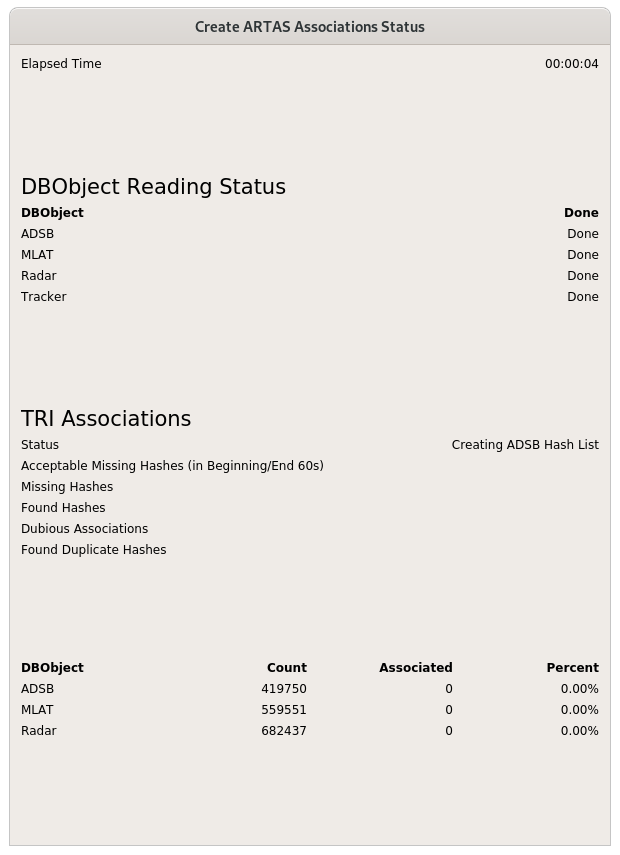
\includegraphics[width=11cm]{figures/artas_assoc_status.png}
  \caption{Associate ARTAS TRIs tatus}
\end{figure}

When the calculation of the ARTAS associations is completed, the assocaition information is written into the database. If there where missed or dubious associations, the user is asked if this is still wanted. Please be aware that it is possible to not save the association information, and to re-run the task with a different configuration.

\begin{figure}[H]
  \center
    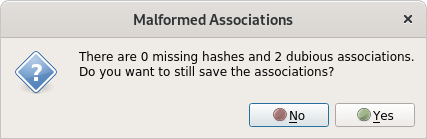
\includegraphics[width=8cm]{figures/artas_assoc_question.png}
  \caption{Associate ARTAS TRIs save question}
\end{figure}

After the assocations are saved, the task is done:

\begin{figure}[H]
  \center
    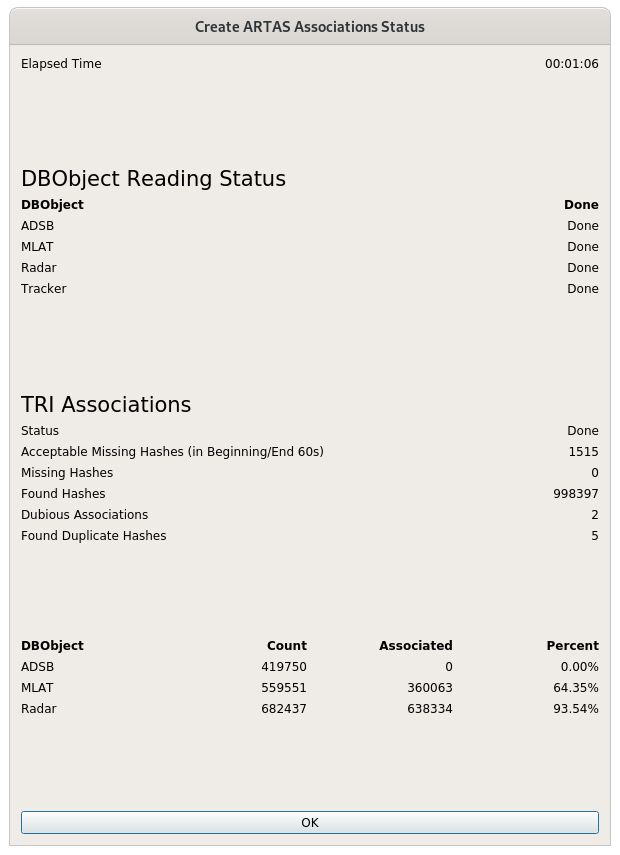
\includegraphics[width=11cm]{figures/artas_assoc_done.png}
  \caption{Associate ARTAS TRIs done}
\end{figure}


